
\subsection{Task 3: On-demand symbolic analysis for DNNs.}
In this task, we will look into the deep neural networks (''inside the box'') to understand its behaviour by using selective static symbolic execution (approximating the model behaviour without running it). 
Through exploring the internal structure of a model, our proposed symbolic on-demand execution can be used to (1) perform \textbf{model certification} or (2) conduct \textbf{structural tuning} to transform the model based on stakeholders' requirements (e.g., making trade-offs such as producing and certifying a model with high precision rather than high recall). 
Our symbolic analysis translates input, output and the neural network into symbolic constraints (rather than exercising their concrete values), so that the user-specified properties can be certified as solving a satisfiability problem.

Inspired by our previous efforts in demand-driven static analysis~\cite{sui2018value,sui2016svf}, this work aims to encode the network dependence rather than code dependence into constraints based on user requirement for fast symbolic certification by employing the idea of \emph{weak-preconditions} and \emph{strong-preconditions}~\cite{sui2016eliminating}. 
Unlike the single-aim driven approach (e.g., accelerating constraint solving by eliminating repeated structures via minimization~\cite{chen2021faster}), our symbolic analysis can also provide a trade-off design to guide stackholders to tune a model into their favourable ones.

\textbf{Symbolic analysis for DNNs.}
To conduct our symbolic certification, we define the following grammar of our constraint specification to formulate the input, output and internal neural network as a conjunction of clauses. 
\begin{equation}\label{eq:constraints}
\begin{array}{rcl}
    C_{com} & \rightarrow & C_{single}\ |\ C_{single} \wedge C_{com},   \\
    C_{single}&  \rightarrow &E < E\ |\ E \le E\ |\ E > E\ |\ E \ge E\ |\ E = E \ |\ E = \sigma(E) \ |\ E = E + E \ |\ E=E* E, \\
     E & \rightarrow & x_i\ |\ y_j\ |\ c\in\mathbb{R}.
\end{array}
\end{equation}
Here $C_{com}$ represents the combined constraint of one or more $C_{single}$ clauses, with each clause representing a single comparison between two entities $E$s, where $E$ is either a variable (e.g., $x_i$ as the $i$-th feature of the input $x$ or an output class $y_j$) or a constant (e.g., $c$).
A $k-$layer neural network can be represented as a compositional function $f(x) = f^k\circ f^{k-1}\circ \dots \circ f^1(x)$. 
The input of the $i+1$-th layer is from the output $h_i$ of $i$-th layer ($h_0$ denotes the original input $x$ to 1st layer). 
\[ h_{i+1} = f^{i+1}(h_{i}) = \sigma_{i}(h_{i}W_{i} + b_{i}), \]
where $\sigma_i$ is the activation function (e.g., ReLU), $W_i$ is the weight matrices, and $b_i$ is the bias value at $i$-th layer of the neural network.

\begin{wrapfigure}{r}{0.5\linewidth}
    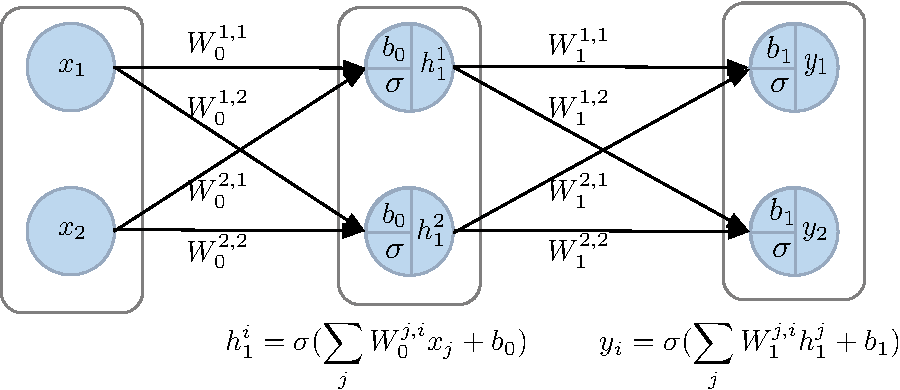
\includegraphics[width=\linewidth]{fig/RP_TASK3_neuralStructure.pdf}
     \caption{\footnotesize Constraints for a tiny  feedforward neural network.}
    \label{fig:neuralStructure}
\end{wrapfigure}

Let us take a look at a certification example using a tiny neural network in Figure~\ref{fig:neuralStructure}. 
A specific input can be expressed as a conjunct clause in the constraint $C_{in}(x_1 < 0.2 \wedge x_2 < 0.5)$, and the neural network is a legitimate model if it can always yield user desired output $C_{out}(y_1 > y_2)$. 
The neural network can be represented as $C_{f}= \bigwedge\limits_{i=1}^2{\sigma(\sum_{j=1}^2W_1^{j,i}h_1^j+b_1)}$.
Finally, a conjunction of constraints $C_{in} \wedge C_{f} \wedge C_{out}$ is used to symbolically execute the model to validate whether the neural network can produce expected output $y$ given the input $x$. 
The constraints can be resolved using an SMT solver (e.g., Z3~\cite{moura2008z3}) to return a satisfactory (certified) result if no counterexample that violates the constraints is found or an unsatisfied result otherwise. 
%Hence, a model is certified by user requirement (expected output) if no counterexample is found. 


\textbf{On-demand certification.} We aim to enforce user-specified properties as input and/or output constraints to enable property-driven certification by employing the idea of weakest precondition and strongest postcondition. 
An input $C_{in}$ to a neural network can be seen as the  precondition and the output $C_{out}$ can be seen as the postcondition.
We say that a constraint $C_{1}$ is stronger than $C_{2}$ if $C_{1}\Rightarrow C_{2}$. 
For example, $x > 0$ is stronger than $x > -1$ or $x > -1$ is weaker than $x > 0$. 
For each incoming constraint $C_{in}$ to the network, there can be many $C_{in}$ such that $C_{in}\wedge C_{f} \wedge C_{out}$ is satisfiable. 
Given any $C_{in}$, the weakest condition $wp(C_{f}, C_{out})$ always satisfy $C_{in} \Rightarrow wp(C_{f}, C_{out})$ such that the output $C_{out}$ holds. 
Obtaining the weakest precondition would measure the model's robustness/tolerance to the input perturbations. On the other  extreme, the strong postcondition $sp(C_{in}, C_{f})$ such that any $C_{out}$ would satisfy $sp(C_{in}, C_{f}) \Rightarrow C_{out}$ provides us the strongest restriction on the output. 
For the use case scenario which balancing between precision and recall, a weaker input constraint can have a better coverage hence a better recall, while a stronger output constraint tends to yield a better precision. 

Of course, obtaining either one of the two extremes (weakest and strongest conditions) can be challenging and impractical in practice since finding them is costly. However, guided by the idea of strongest and weakest conditions, we could certify the model with user-specified properties to understand and report the capability of the model based on user expectations. 
For example, given the expected output, we can quantitatively measure the robustness or resilience of a model to input perturbations by reasoning about the weaker conditions of the original input. For another example, given a fixed input, we could reasoning about a stronger output constraint than the original output to boost the precision by adjusting the  probability distribution of all possible outputs.

%Of course, obtaining  either one of the two extremes (illustrated in Figure~\ref{fig:certify}) can be challenging and impractical in reality since pruning itself is costly to find the weakest precondition and strongest postcondition. 


\begin{wrapfigure}{r}{7cm}
    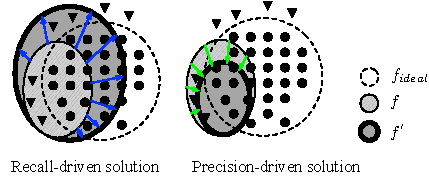
\includegraphics[scale=1]{fig/certify.pdf}
     \caption{\footnotesize On-demand symbolic analysis to guide model tuning based on stackholders' requirement. The first example denotes a recall-driven solution (with compromise on precision but not recall) and the second example denotes a precision-driven solution (with compromise on recall but not precision).}
    \label{fig:certify}
\end{wrapfigure}

\textbf{On-demand structural tuning.}
Model tuning can help obtain a desired model if the original one is unfavourable to a stackholder. 
For example, training and certifying large-scale DNN models on resource-limited edge devices, such as smartphones and wearable devices are very costly. Driven by efficiency, structural pruning can remove redundant neurons with much less constraints to accelerate the model certification or resource-limited training. More importantly, our symbolic analysis allows a negotiable decision making process to tune a desired model to meet a stackholder's requirement.

%For example, \textcolor{red}{moderate-sized networks trained for xxx task can contain over 100,000 neurons and xxx single constraints}.
%In this task, we aim to tune a DNN model based on the properties (e.g., precision or recall) required stackholders. %hence significantly benefiting both the training and certification process.

Figure~\ref{fig:certify} demonstrates the idea of our approach using a simple binary classification example.
An ideal classifier $f_{ideal}$ (as depicted using a dotted circle) has full precision and recall to correctly identify all positive samples (dots) and excluding all negative samples (triangles).
In practice, ${f}$ represents the imperfect model we would like to certify.
We aim to tune ${f}$ to $f'$ by pruning/adding some neurons and their connected edges to relax/tighten the constraints based on user needs. For example, the recall-driven request in which the solution space becomes conservatively larger while the counterexample search space is shrunk; while the precision-driven request in which the solution space becomes aggressively smaller for a fast convergence during constraint solving. 


\begin{comment}
Given an input $x$ in the input space, a DNN model $y=f_\theta(x)$ essentially maps $x$ to a solution space (depicted as the white circle), which is a subarea of the entire output space.
The solution space represents that any solution in the white circle outputs $y$ in terms of ranking $y\in\mathbb{Y}$ as the highest probability among all others in $\mathbb{Y}$. 
Given a perturbed $x'$ on $x$ in the input space, a robust model $f_\theta$ can correctly map $x'$ to the same solution space in the output space. 
The robustness can be verified by finding counterexamples in the grey area by solving the constraints (Equation~\ref{eq:constraints}) of the model.
\end{comment}


\begin{comment}
\textbf{Approximate model pruning.}
We aim to explore two approximate pruning approaches using (1) a new path-based typestate (i.e., property simulation) analysis~\cite{li2022path} for approximate pruning by exercising the paths on the directed acyclic network graph, and (2) a masked-pruning approach to determine the likely redundancy based on the user-specified property.
\emph{(1) Path-based pruning}. Given the encoded constraint $C_{in} \wedge C_{f} \wedge C_{out}$ for the network $f$, the path-based approach dismantle encoding based on the paths of the network, (i.e., $C_{in} \wedge (\bigwedge\limits_{p\in paths(f)} C_p) \wedge C_{out}$) and then conduct property-driven constraint analysis by sampling some of the important paths. For each sample path $p$, we aim to transform its constraint $C_p$ to $C_p'$ guided by the properties (e.g., weakest condition $C_{in}$ and strongest $C_{out}$) such that $C_p'$ reflects a pruned or constraint transformed neurons on the path to produce a desired user-required network. 


%Current model pruning focuses on accuracy guarantee via structural and weight pruning techniques. However, few attention has been paid to the model pruning for robust networks. This project aims at structural pruning on the robust model via a generic structural pruning framework. 

%Notations and definitions for model pruning are provided firstly.  Let $n$ be the total number of layers, $m_i$ denotes the number of neurons in the layer $l^i$, the robust deep learning model $\mathcal{M}'$ can be presented as $\mathcal{M}'= \langle L, W, b, \Phi \rangle$, where $L=\{ l^{i}\ |\ 0\leq i\le n \}$ is a set of layers and $l^0$ denotes the input layer, $W=\{w^i\ |\ w^i\in\mathbb{R}^{m_{i-1}\times m_{i}}, 1\le i\le n \}$ is the set of weight matrices, $\ b=\{b^i\ |\ b^i\in\mathbb{R}^{m_i}, 1\le i\le n \}$ is the set of bias vectors, and $\Phi=\{\phi^i\ |\ 1\le i\le n\}$ is the set of activation functions. Given a model $\mathcal{M}'$, the output vector $o^{i+1}\in\mathbb{R}^{m_{i+1}}$ of layer $l^{i+1}$ ($0\le i\le n-1$) can be defined as:
%\begin{equation}
%    o^{i+1} = \phi^{i+1}(o^{i}\times w^{i+1} + b^{i+1}).
%\end{equation}

\emph{(1) Masked-pruning.} Structural pruning aims to remove the redundancy structures in a deep neural network. For layer-wise pruning, the target of structural pruning can be formalized to find a pruning mask $a^i=\{a^{i,j}\ |\ a^{i,j}\in\{0,1\}\}^{m_i}_{j=1}$ for layer $l^i$ to satisfy Equation~\eqref{eq:l_pruning}:
 \begin{equation}\label{eq:l_pruning}
 h_{i+1}=\sigma_{i+1}(h_i\times W_{i+1}+b_{i+1})\simeq \sigma_{i+1}(h_i\circ a_i\times \hat{W}_{i+1}+\hat{b}_{i+1}), 
 \end{equation}
 where $\circ$ denotes the Hadamard product, $\hat{w}^{i+1}$ and $\hat{b}^{i+1}$ denotes new weights and bias to be updated after the pruning. Here, the objective for the pruning is:
 \begin{equation}\label{eq:pruning_target}
     \min(\frac{\beta}{2m_{i+1}}\|h_{i+1} - \sigma_{i+1}(h_i\circ a_i\times \hat{W}_{i+1}+\hat{b}_{i+1})\|^2_2),
 \end{equation}
 where $\beta$ denotes the scaling factor.


 To address the optimization problem in Equation~\eqref{eq:pruning_target}, previous studies~\cite{luo2017thinet, jiang2018efficient} focus on given pruning rates and select the pruning neurons by iteratively updating the binary mask via the greedy selection and weight update. In this project, we propose an auto-encoder-based structural pruning method to learn a binary mask for automatic layer-wise model pruning in Figure~\ref{fig:task3_pruning}. According to Figure~\ref{fig:task3_pruning}, we conduct layer-wise pruning on robust model $\mathcal{M}'$ through the reconstruction of the weight matrix of two adjacent layers. Specifically, motivated by Equation~\eqref{eq:l_pruning}, we use an encoder network to model the mask process and a decoder network to recover the input $o_i$ for layer $l^i$. Here, we iteratively train the binary mask for each layer in model $\mathcal{M}'$ from bottom to top. 

  
  \begin{figure}[!t]
    \centering
    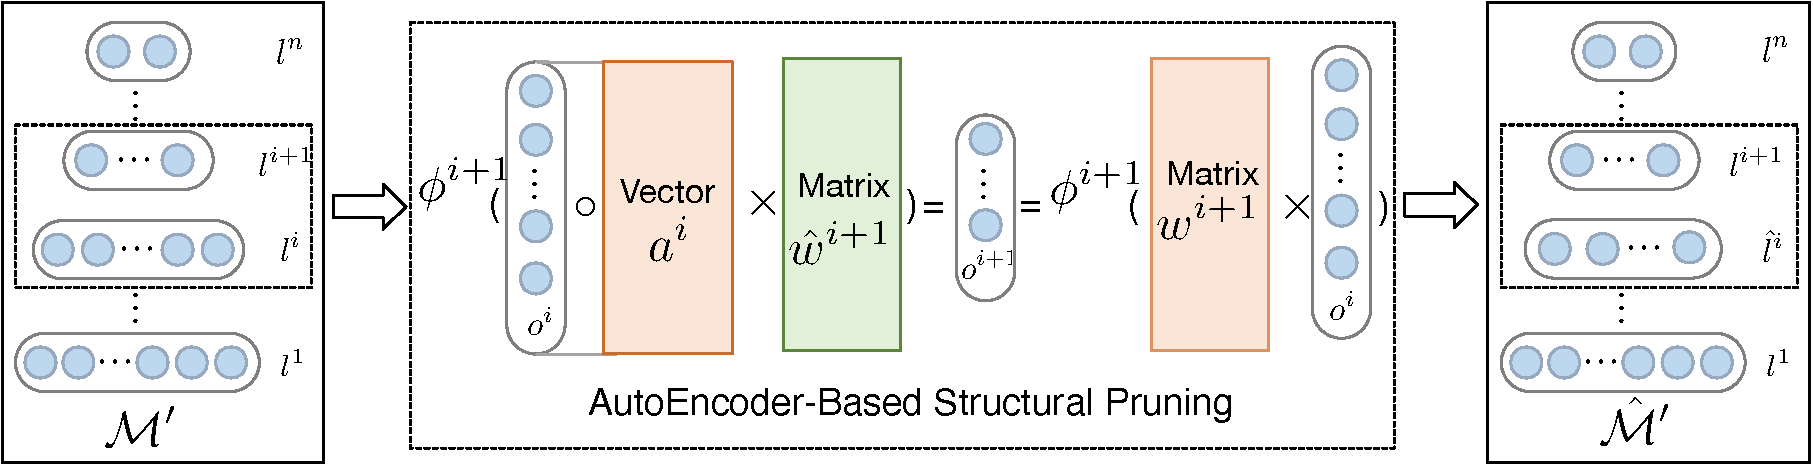
\includegraphics[width=0.9\textwidth]{fig/RP_TASK3_pruning.pdf}
    \caption{Model pruning for robust DNN.}
    \label{fig:task3_pruning}
\end{figure}

 Compared with previous methods, our proposed one enables two advantages: (1) Our method selects the pruning neurons automatically without a specified pruning rate; (2) The by-product of the structure $\hat{w}^{i+1}$ for layer $l^i$ is performance-preserving and no extra fine-tuning process is required. Here, considering the input $a^i$ of this auto-encoder is data-related ($a^0$ in the first layer is the input data), the parameters in this autoencoder can be updated by the training set. Regarding the optimization-enabled update process, the objective function is composed of the following parts:
 
\begin{itemize}
    \item Reconstruction loss. Reconstruction loss aims to guarantee the minimum distance between the encoder and decoder outputs. We can present the Reconstruction loss as:
    \begin{equation}\label{eq:reconstruction_loss}
        \mathcal{L}_{RC} =  
     \frac{\alpha}{2m_{i+1}}\|\sigma^{i+1}(o^i\times w^{i+1}+b^{i+1}) - \sigma^{i+1}(o^i\circ a^i\times \hat{w}^{i+1}+\hat{b}^{i+1})\|^2_2,
    \end{equation}
    where $\alpha$ denotes the scaling factor.
    \item Maximum pruning loss. Maximum pruning loss removes the weights in a layer to the utmost extent. Considering the pruning mask is a binary vector, We can present the maximum pruning loss as:
    \begin{equation}
        \mathcal{L}_{MP} = \beta \sum_{j=1}^{m_{i+1}} a^{i,j},
    \end{equation}
    where $\beta$ denotes the balancing coefficient.
    \item Performance-preserving loss. To maintain the robustness of the robust $\mathcal{M}'$, the trained encode vector is expected to be close to the initial encoder vector $o^{i+1}$. We  can present the loss as:
    \begin{equation}
        \mathcal{L}_{PP} =  \frac{\gamma}{2m_{i+1}}\|o^{i+1} - \sigma^{i+1}(o^i\circ a^i\times \hat{w}^{i+1}+\hat{b}^{i+1})\|^2_2,
    \end{equation}
    where $\gamma$ denotes the scaling factor.
\end{itemize}

Finally, the loss for the optimization $\mathcal{L}_{pruning}$ is:
\begin{equation}
    \mathcal{L}_{pruning} = \mathcal{L}_{RC}+\mathcal{L}_{MP}+\mathcal{L}_{PP}.
\end{equation}

Noted that original binary network is hard to converge, here soft mask technique is utilized ($a^i=\{a^{i,j}|a^{i,j}\in \mathcal{R}^{m_i}_{j=1}, 0\le a^{i,j}\le 1$). In addition, two-step optimization from FISTA~\cite{denton2014exploiting} is introduced to solve the optimization of $a^i$ and $\hat{w}^i$.
After the iteration of the structural pruning, we can obtain a pruned model $\mathcal{M}^{''}$, where the new structure in layer $l^i$ and the corresponding weights $\hat{w}^{'}$ are from the trained auto-encoder. In this project, we will further explore the formal verification techniques in \textbf{Task 4} to verify the preserved robustness of the pruned model $\mathcal{M}^{''}$ and certificate it with a quantified score.


\end{comment}